% 使用书页原图的高清修复版；下方旧 TikZ 代码保留备查，不再执行。
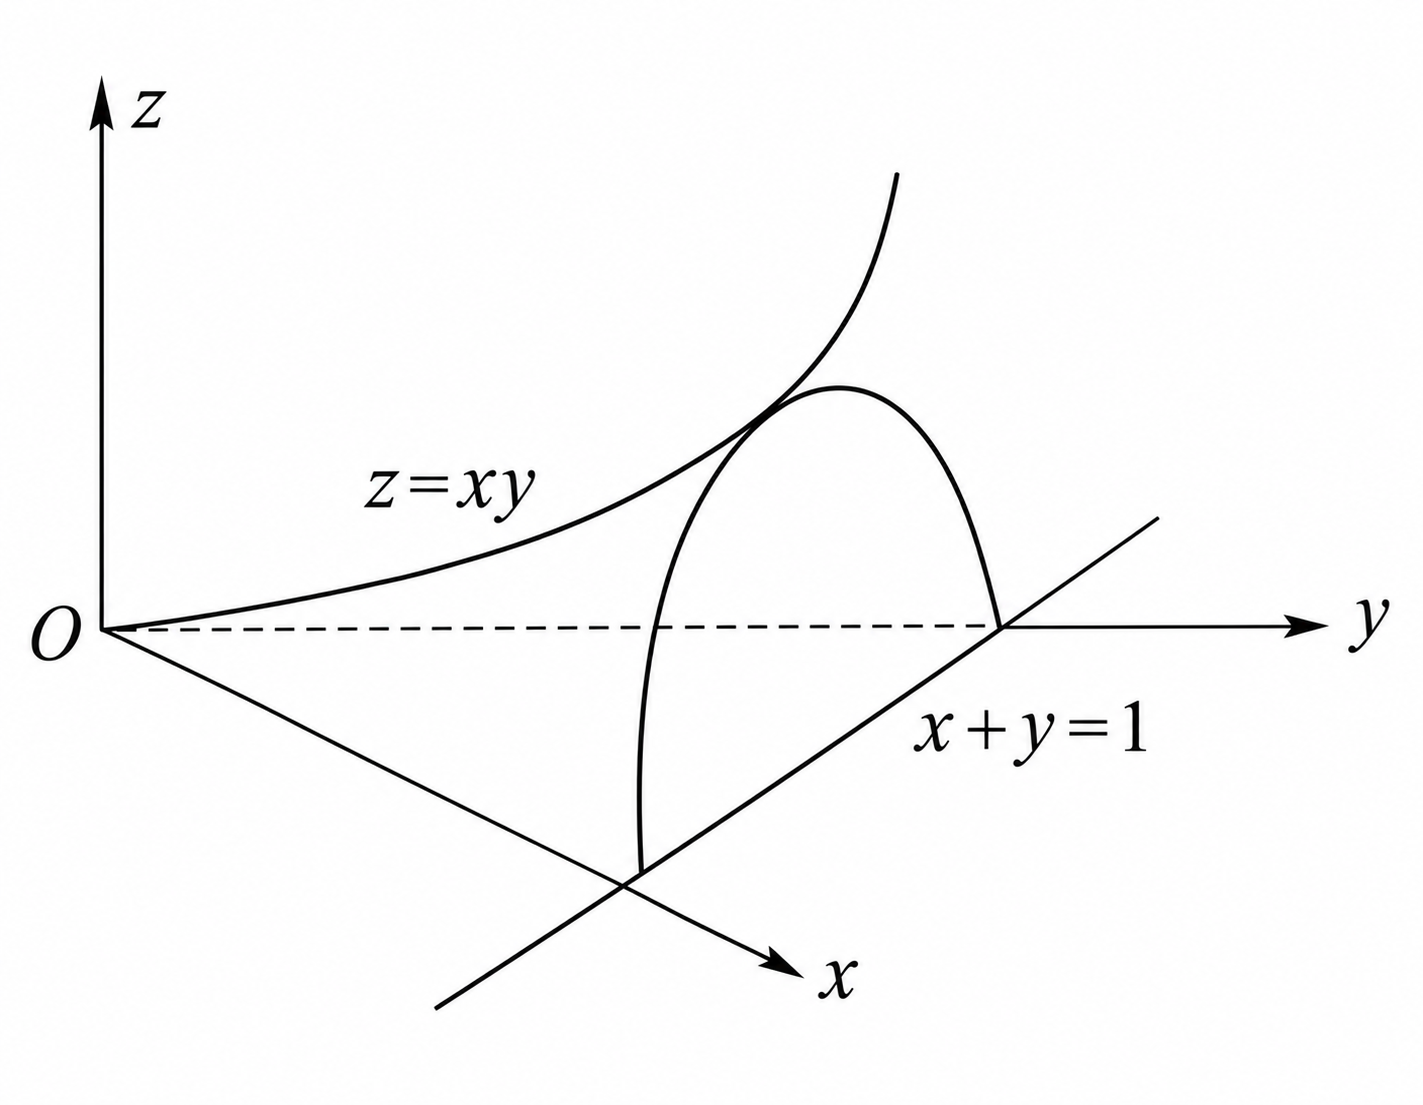
\includegraphics[width=0.45\textwidth]{figure/P2/sec2_metal_source_hd.png}
\endinput
% z=xy、x+y=1 与 z=0 所围区域。
\begin{tikzpicture}[
  x={(2cm,-1.1cm)},y={(2.4cm,.2cm)},z={(0cm,3cm)},
  >=Stealth,font=\small,line join=round]
  \draw[->] (0,0,0) -- (1.35,0,0) node[below right] {$x$};
  \draw[->] (0,0,0) -- (0,1.35,0) node[right] {$y$};
  \draw[->] (0,0,0) -- (0,0,.85) node[above] {$z$};
  \node[left] at (0,0,0) {$O$};
  \draw[line width=.65pt] (1,0,0) -- (0,1,0);
  \draw[line width=.75pt,domain=0:1,samples=45,variable=\t]
    plot ({\t},{1-\t},{\t*(1-\t)});
  \foreach \t in {.25,.5,.75}{
    \draw[gray,thin] (\t,0,0) -- (\t,{1-\t},{\t*(1-\t)});
    \draw[dashed,thin] (\t,{1-\t},0) -- (\t,{1-\t},{\t*(1-\t)});
  }
  \node[above] at (.18,.25,.42) {$z=xy$};
  \node[right] at (.75,.25,.04) {$x+y=1$};
\end{tikzpicture}
